\section{Calculus and Vector-Valued Functions}\label{sec:vvf_calc}

The previous section introduced us to a new mathematical object, the vector-valued function. We now apply calculus concepts to these functions. We start with the limit, then work our way through derivatives to integrals.

\subsection{Limits of Vector-Valued Functions}

The initial definition of the limit of a vector-valued function is a bit intimidating, as was the definition of the limit in \autoref{def:limit}. The theorem following the definition shows that in practice, taking limits of vector-valued functions is no more difficult than taking limits of real-valued functions.

\begin{definition}[Limits of Vector-Valued Functions]\label{def:vvf_limit}
Let $I$ be an open interval containing $c$, and let $\vec r(t)$ be a vector-valued function defined on $I$, except possibly at $c$. %Let a vector-valued function $\vec r(t)$ be given, defined on an open interval $I$ containing $c$. 
The \textbf{limit of $\vec r(t)$, as $t$ approaches $c$, is $\vec L$}, expressed as 
\[\lim_{t\to c} \vec r(t) = \vec L,\]
means that given any $\epsilon>0$, there exists a $\delta>0$ such that for all $t\neq c$, if $\abs{t-c}<\delta$, we have $\norm{\vec r(t) - \vec L} < \epsilon.$
\index{vector-valued function!limits}\index{limit!of vector-valued functions}
\end{definition}

Note how the measurement of distance between real numbers is the absolute value of their difference; the measure of distance between vectors is the vector norm, or magnitude, of their difference.

\begin{theorem}[Limits of Vector-Valued Functions]\label{thm:vvf_limit}
\index{vector-valued function!limits}\index{limit!of vector-valued functions}%
\mbox{}\\[-2\baselineskip]\begin{enumerate}
	\item Let $\vec r(t) =\bracket{\,f(t),g(t)\,}$ be a vector-valued function in $\mathbb{R}^2$ defined on an open interval $I$ containing $c$. Then
\[\lim_{t\to c} \vec r(t) =\bracket{\lim_{t\to c}f(t)\, , \,\lim_{t\to c} g(t)}.\]
	\item Let $\vec r(t) =\bracket{\,f(t),g(t),h(t)\,}$ be a vector-valued function in $\mathbb{R}^3$ defined on an open interval $I$ containing $c$. Then 
\[
\lim_{t\to c} \vec r(t)
=\bracket{\lim_{t\to c}f(t)\, , \,\lim_{t\to c} g(t)\,, \,\lim_{t\to c} h(t)}
\]
\end{enumerate}
If any of the component limits do not exist, then $\ds\lim_{t\to c} \vec r(t)$ does not exist.
\end{theorem}

\autoref{thm:vvf_limit} states that we compute limits component-wise.

\begin{example}[Finding limits of vector-valued functions]\label{ex_vvflimit1}
Let $\ds\vec r(t) =\bracket{\frac{\sin t}{t},\, t^2-3t+3,\,\cos t}.$ Find $\ds \lim_{t\to 0}\vec r(t)$.
\solution
We apply the theorem and compute limits component-wise.
\begin{align*}
\lim_{t\to0} \vec r(t) &=\bracket{\lim_{t\to 0}\frac{\sin t}{t}\, , \, \lim_{t\to 0} t^2-3t+3\, , \, \lim_{t\to 0} \cos t}\\
			&=\bracket{1,3,1}.
\end{align*}
\end{example}

\subsection{Continuity}

\begin{definition}[Continuity of Vector-Valued Functions]\label{def:vvf_continuity}
Let $\vec r(t)$ be a vector-valued function defined on an open interval $I$ containing $c$.
\index{vector-valued function!continuity}\index{continuous function!vector-valued}
\begin{enumerate}
	\item $\vec r(t)$ is \textbf{continuous at $c$} if $\ds \lim_{t\to c} \vec r(t) = \vec r(c)$.
	\item	If $\vec r(t)$ is continuous at all $c$ in $I$, then $\vec r(t)$ is \textbf{continuous on $I$.}
\end{enumerate}
\end{definition}

We again have a theorem that lets us evaluate continuity component-wise.

\begin{theorem}[Continuity of Vector-Valued Functions]\label{thm:vvf_continuity}
Let $\vec r(t)$ be a vector-valued function defined on an open interval $I$ containing $c$. Then $\vec r(t)$ is continuous at $c$ if, and only if, each of its component functions is continuous at $c$.
\index{vector-valued function!continuity}\index{continuous function!vector-valued}
\end{theorem}

\begin{example}[Evaluating continuity of vector-valued functions]\label{ex_vvflimit2}
Let $\ds\vec r(t) =\bracket{\frac{\sin t}{t},\, t^2-3t+3,\,\cos t}.$ Determine whether $\vec r$ is continuous at $t=0$ and $t=1$.
\solution
While the second and third components of $\vec r(t)$ are defined at $t=0$, the first component, $(\sin t)/t$, is not. Since the first component is not even defined at $t=0$, $\vec r(t)$ is not defined at $t=0$, and hence it is not continuous at $t=0$.

At $t=1$ each of the component functions is continuous. Therefore $\vec r(t)$ is continuous at $t=1$.
\end{example}

\subsection{Derivatives}

Consider a vector-valued function $\vec r$ defined on an open interval $I$ containing $t_0$ and $t_1$. We can compute the displacement of $\vec r$ on $[t_0,t_1]$, as shown in \autoref{fig:vvfderiv_intro}(a). Recall that dividing the displacement vector by $t_1-t_0$ gives the average rate of change on $[t_0,t_1]$, as shown in (b).

\noindent\begin{minipage}[t]{\linewidth}\noindent%
\captionsetup{type=figure}%
\flushinner{%
\begin{tabular}{cc}
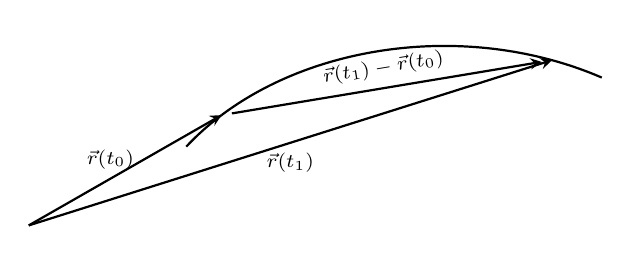
\begin{tikzpicture}[>=stealth]
 \draw [thick,draw={\colorone}]
  (2,1) arc [x radius=4,y radius=3,start angle=145,end angle=135] node (A) {};
 \draw [thick,draw={\colorone}]
  (A.center) arc [x radius=4,y radius=3,start angle=135,end angle=70] node (B) {};
 \draw [thick,draw={\colorone}]
  (B.center) arc [x radius=4,y radius=3,start angle=70,end angle=60];
 \draw [thick,->] (0,0) -- (A.center) node [left,pos=.6] {\scriptsize $\vec r(t_0)$};
 \draw [thick,->] (0,0)
  -- (B.center) node [below,pos=.5] {\scriptsize $\vec r(t_1)$};
 \draw [->,thick,draw={\colortwo}] (A)
  --(B) node [above,black,pos=.5,sloped] {\scriptsize $\vec r(t_1)-\vec r(t_0)$};
\end{tikzpicture}
&
\begin{tikzpicture}[>=stealth]
 \draw [thick,draw={\colorone}]
  (2,1) arc [x radius=4,y radius=3,start angle=145,end angle=135] node (A) {};
 \draw [thick,draw={\colorone}]
  (A.center) arc [x radius=4,y radius=3,start angle=135,end angle=70] node (B) {};
 \draw [thick,draw={\colorone}]
  (B.center) arc [x radius=4,y radius=3,start angle=70,end angle=60];
 \draw [thick,->] (0,0) -- (A.center) node [left,pos=.6] {\scriptsize $\vec r(t_0)$};
 \draw [thick,->] (0,0)
  -- (B.center) node [below,pos=.5] {\scriptsize $\vec r(t_1)$};
 \draw [->,thick,draw={\colortwo}] (A.center)--($(A)!1.2!(B)$)
  node [above,black,pos=.99,] {$\frac{\vec r(t_1)-\vec r(t_0)}{t_1-t_0}$};
 \draw [->,thick,draw={\colortwo}] (A.center)--($(A)!.4!29:(B)$)
  node [above,black] {\scriptsize $\vec r\,'(t_0)$};
\end{tikzpicture}
\\(a) & (b)
\end{tabular}}
\caption{Illustrating displacement, leading to an understanding of the derivative of vector-valued functions.}
\label{fig:vvfderiv_intro}
\end{minipage}

The \textbf{derivative} of a vector-valued function is a measure of the \emph{instantaneous} rate of change, measured by taking the limit as the length of $[t_0,t_1]$ goes to 0. Instead of thinking of an interval as $[t_0,t_1]$, we think of it as $[c,c+h]$ for some value of $h$ (hence the interval has length $h$).  The \emph{average} rate of change is 
\[\frac{\vec r(c+h)-\vec r(c)}{h}\]
for any value of $h\neq0$. We take the limit as $h\to0$ to measure the instantaneous rate of change; this is the derivative of $\vec r$.

%We begin with a definition of the derivative that is very similar to \autoref{def:the_derivative}.

\begin{definition}[Derivative of a Vector-Valued Function]\label{def:vvf_derivative}
Let $\vec r(t)$ be continuous on an open interval $I$ containing $c$.
\index{vector-valued function!derivatives}\index{derivative!vector-valued functions}
\begin{enumerate}
	\item The derivative of $\vec r$ at $t=c$ is the vector
	\[\vrp (c) = \lim_{h\to 0} \frac{\vec r(c+h) - \vec r(c)}{h}.\]
	\item	The derivative of $\vec r$ is the vector-valued function
	\[\vrp (t) = \lim_{h\to 0} \frac{\vec r(t+h) - \vec r(t)}{h}.\]
\end{enumerate}
\end{definition}

\mnote{Alternate notations for the derivative of $\vec r$ include:
\[\vrp(t) = \frac{d}{dt}\bigl(\,\vec r(t)\,\bigr) = \frac{d\vec r}{dt}.\]}

If a vector-valued function has a derivative for all $c$ in an open interval $I$, we say that $\vec r(t)$ is \textbf{differentiable} on $I$.

Once again we might view this definition as intimidating, but recall that we can evaluate limits component-wise. The following theorem verifies that this means we can compute derivatives component-wise as well, making the task not too difficult.

\begin{theorem}[Derivatives of Vector-Valued Functions]\label{thm:vvf_deriv}
\index{vector-valued function!derivatives}\index{derivative!vector-valued functions}
\mbox{}\\[-2\baselineskip]\begin{enumerate}
	\item Let $\vec r(t) =\bracket{\, f(t), g(t)\,}$. Then 
	\[\vrp(t) =\bracket{\, \fp(t), g\primeskip'(t)\,}.\]
	\item Let $\vec r(t) =\bracket{\, f(t), g(t), h(t)\,}$. Then
	\[\vrp(t) =\bracket{\, \fp(t), g\primeskip'(t), h\primeskip'(t)\,}.\]
\end{enumerate}
If any of the component derivatives do not exist, then $\vrp(t)$ does not exist.
\end{theorem}

\youtubeVideo{238wiC0U7NE}{Limit and Derivative of Vector Function}

\mtable[-1in]{Graphing the derivative of a vector-valued function in \autoref{ex_vvflimit3}.}{fig:vvflimit3}{%
\begin{tikzpicture}[>=stealth]
\begin{axis}[width=1.16\marginparwidth,tick label style={font=\scriptsize},
axis y line=middle,axis x line=middle,name=myplot,
ymin=-2.2,ymax=2.2,xmin=-4.54,xmax=4.54]
\addplot [thick,draw={\colorone}, smooth,domain=-2:2,samples=20] ({x^2},{x});
\draw (axis cs:2,1.7) node {\scriptsize $\vec r(t)$};
\draw [thick,draw={\colortwo}] (axis cs: -4,1) -- (axis cs:4,1)
 node [below,pos=.9,black]{\scriptsize $\vec r\,'(t)$};
\draw [thick,draw={\colortwo},->] (axis cs: -2,1) -- (axis cs:-1.99,1);
\draw [thick,->,draw={\colorone}] (axis cs:1,-1) -- (axis cs:0.9801,-.99);
\end{axis}
\node [right] at (myplot.right of origin) {\scriptsize $x$};
\node [above] at (myplot.above origin) {\scriptsize $y$};
\end{tikzpicture}
\\[5pt](a)\\[10pt]
\begin{tikzpicture}[>=stealth]
\begin{axis}[width=1.16\marginparwidth,tick label style={font=\scriptsize},
axis y line=middle,axis x line=middle,name=myplot,
ymin=-2.2,ymax=2.2,xmin=-4.54,xmax=4.54]
\addplot [thick,draw={\colorone}, smooth,domain=-2:2,samples=20] ({x^2},{x});
\draw [thick,->,draw={\colortwo}] (axis cs: 0,0) -- (axis cs:2,1)
 node [shift={(15pt,0)},pos=.6,black]{\scriptsize $\vec r\,'(1)$};
\draw [thick,->,draw={\colortwo}] (axis cs: 1,1) -- (axis cs:3,2)
 node [left,pos=.8,black]{\scriptsize $\vec r\,'(1)$};
\draw [thick,->,draw={\colorone}] (axis cs:1,-1) -- (axis cs:0.9801,-.99);
\end{axis}
\node [right] at (myplot.right of origin) {\scriptsize $x$};
\node [above] at (myplot.above origin) {\scriptsize $y$};
\end{tikzpicture}
\\[5pt](b)}

\begin{example}[Derivatives of vector-valued functions]\label{ex_vvflimit3}
Let $\vec r(t) =\bracket{t^2,t}$. 
\begin{enumerate}
	\item Sketch $\vec r(t)$ and $\vrp(t)$ on the same axes.
	\item	Compute $\vrp(1)$ and sketch this vector with its initial point at the origin and at $\vec r(1)$.
\end{enumerate}
\solution
\begin{enumerate}
\item	\autoref{thm:vvf_deriv} allows us to compute derivatives component-wise, so
\[\vrp(t) =\bracket{2t, 1}.\]
$\vec r(t)$ and $\vrp(t)$ are graphed together in \autoref{fig:vvflimit3}(a). Note how plotting the two of these together, in this way, is not very illuminating. When dealing with real-valued functions, plotting $f(x)$ with $\fp(x)$ gave us useful information as we were able to compare $f$ and $\fp$ at the same $x$-values. When dealing with vector-valued functions, it is hard to tell which points on the graph of $\vrp$ correspond to which points on the graph of $\vec r$.

\item	We easily compute $\vrp(1) =\bracket{2,1}$, which is drawn in \autoref{fig:vvflimit3} with its initial point at the origin, as well as at $\vec r(1) =\bracket{1,1}.$ These are sketched in \autoref{fig:vvflimit3}(b).
\end{enumerate}
\end{example}

\ifthenelse{\boolean{in_threeD}}{%
\mtable{Viewing a vector-valued function and its derivative at one point.}{fig:vvflimit4}{%
\myincludeasythree{width=.7\marginparwidth,
3Droll=-0.5856992334166129,
3Dortho=0.004399999976158142,
3Dc2c=0.6354137063026428 0.6317671537399292 0.4439816176891327,
3Dcoo=-18.837804794311523 -8.740551948547363 60.22870635986328,
3Droo=150.0000027221829}{width=.7\marginparwidth}{figures/figvvflimit4_3D}}%
}{% not in threeD
\mtable[-3\baselineskip]{Viewing a vector-valued function and its derivative at one point, from two different perspectives.}{fig:vvflimit4}{%
\myincludegraphics[width=.7\marginparwidth]{figures/figvvflimit4_3D}
\\(a)\\
\myincludegraphics[width=.7\marginparwidth]{figures/figvvflimit4a_3D}
\\(b)}%
}% ends whole if-then-else

\begin{example}[Derivatives of vector-valued functions]\label{ex_vvflimit4}
Let $\vec r(t) =\bracket{\cos t, \sin t, t}$. Compute $\vrp(t)$ and $\vrp(\pi/2)$. Sketch $\vrp(\pi/2)$ with its initial point at the origin and at $\vec r(\pi/2)$.
\solution
We compute $\vrp$ as $\vrp(t) =\bracket{-\sin t, \cos t, 1}$. At $t= \pi/2$, we have $\vrp(\pi/2) =\bracket{-1,0,1}$. \autoref{fig:vvflimit4}
\ifthenelse{\boolean{in_threeD}}{shows a graph of $\vec r(t)$,}{shows two graphs of $\vec r(t)$, from different perspectives,}
with $\vrp(\pi/2)$ plotted with its initial point at the origin and at $\vec r(\pi/2)$.
\end{example}

In Examples \ref{ex_vvflimit3} and \ref{ex_vvflimit4}, sketching a particular derivative with its initial point at the origin did not seem to reveal anything significant. However, when we sketched the vector with its initial point on the corresponding point on the graph, we did see something significant: the vector appeared to be \emph{tangent} to the graph. We have not yet defined what ``tangent'' means in terms of curves in space; in fact, we use the derivative to define this term.

\begin{definition}[Tangent Vector, Tangent Line]\label{def:vector_tangent}
Let $\vec r(t)$ be a differentiable vector-valued function on an open interval $I$ containing $c$, where $\vrp(c)\neq \vec 0$.
\index{tangent line}\index{vector-valued function!tangent line}
\begin{enumerate}
	\item A vector $\vec v$ is \textbf{tangent to the graph of $\vec r(t)$ at $t=c$} if $\vec v$ is parallel to $\vrp(c)$.
	\item	The \textbf{tangent line}  to the graph of $\vec r(t)$ at $t=c$ is the line through $\vec r(c)$ with direction parallel to $\vrp(c)$. An equation of the tangent line is 
	\[\vec \ell(t) = \vec r(c) + t\,\vrp(c).\]
\end{enumerate}
\end{definition}

\begin{example}[Finding tangent lines to curves in space]\label{ex_vvfderiv1}
Let $\vec r(t) =\bracket{t,t^2,t^3}$ on $[-1.5,1.5]$. Find the vector equation of the line tangent to the graph of $\vec r$ at $t=-1$.
\solution
To find the equation of a line, we need a point on the line and the line's direction. The point is given by $\vec r(-1) =\bracket{-1,1,-1}$. (To be clear, $\bracket{-1,1,-1}$ is a \emph{vector}, not a point, but we use the point ``pointed to'' by this vector.)

\ifthenelse{\boolean{in_threeD}}{% in threeD
\mtable{Graphing a curve in space with its tangent line.}{fig:vvfderiv1}{%
\myincludeasythree{width=\marginparwidth,
3Droll=0.5961816528018784,
3Dortho=0.00514203542843461,
3Dc2c=0.8352102637290955 0.5152699947357178 0.19214747846126556,
3Dcoo=-5.658682346343994 19.23411750793457 0.2712952494621277,
3Droo=149.99999927774635}{width=\marginparwidth}{figures/figvvfderiv1_3D}}
}{% not in three D
\mtable{Graphing a curve in space with its tangent line.}{fig:vvfderiv1}{%
\myincludegraphics[width=\marginparwidth]{figures/figvvfderiv1_3D}
\\(a)\\[10pt]
\myincludegraphics[width=\marginparwidth]{figures/figvvfderiv1b_3D}
\\(b)}% end mtable
}% ends all of the if-then-else statements

The direction comes from $\vrp(-1)$. We compute, component-wise, $\vrp(t) =\bracket{1,2t, 3t^2}$. Thus $\vrp(-1) =\bracket{1,-2,3}$. 

The vector equation of the line is $\ell(t) =\bracket{-1,1,-1}+ t\bracket{1,-2,3}$. \ifthenelse{\boolean{in_threeD}}{This line and $\vec r(t)$ are sketched in \autoref{fig:vvfderiv1}.}{This line and $\vec r(t)$ are sketched, from two perspectives, in \autoref{fig:vvfderiv1} (a) and (b).}
\end{example}

\begin{example}[Finding tangent lines to curves]\label{ex_vvfderiv3}
Find the equations of the lines tangent to $\vec r(t) =\bracket{t^3,t^2}$ at $t=-1$ and $t=0$.
\solution
We find that $\vrp(t) =\bracket{3t^2,2t}$. At $t=-1$, we have
\[\vec r(-1) =\bracket{-1,1}\quad \text{and}\quad \vrp(-1) =\bracket{3,-2},\]
so the equation of the line tangent to the graph of $\vec r(t)$ at $t=-1$ is
\[\ell(t) =\bracket{-1,1}+ t\bracket{3,-2}.\]
This line is graphed with $\vec r(t)$ in \autoref{fig:vvfderiv3}.

At $t=0$, we have $\vrp(0) =\bracket{0,0}=\vec 0$. This implies that the tangent line ``has no direction.'' We cannot apply \autoref{def:vector_tangent}, hence cannot find the equation of the tangent line.
\end{example}

\mtable[1.5in]{Graphing $\vec r(t)$ and its tangent line in \autoref{ex_vvfderiv3}.}{fig:vvfderiv3}{\begin{tikzpicture}[>=stealth]
\begin{axis}[width=1.16\marginparwidth,tick label style={font=\scriptsize},
axis y line=middle,axis x line=middle,name=myplot,
ymin=-2.96,ymax=2.96,xmin=-3.5,xmax=3.5]
\addplot [thick,draw={\colorone}, smooth,domain=-1.5:1.5,samples=30] ({x^3},{x^2});
\addplot [thick,draw={\colortwo}, smooth,domain=-1:1.5,samples=30] ({3*x-1},{-2*x+1});
\draw (axis cs:2,2) node {\scriptsize $\vec r(t)$};
\draw (axis cs:2,-1.7) node {\scriptsize $\vec \ell(t)$};
\draw [thick,draw={\colorone},->] (axis cs: 1,1) -- (axis cs:1.03,1.02);
\draw [thick,draw={\colortwo},->] (axis cs:2,-1)--(axis cs:2.03,-1.02);
\end{axis}
\node [right] at (myplot.right of origin) {\scriptsize $x$};
\node [above] at (myplot.above origin) {\scriptsize $y$};
\end{tikzpicture}}

We were unable to compute the equation of the tangent line to $\vec r(t)=\bracket{t^3,t^2}$ at $t=0$ because $\vrp(0) = \vec 0$. The graph in \autoref{fig:vvfderiv3} shows that there is a cusp at this point. This leads us to another definition of \textbf{smooth}, previously defined by \autoref{def:smooth} in \autoref{sec:param_eqs}.

\begin{definition}[Smooth Vector-Valued Functions]\label{def:vector_smooth}
Let $\vec r(t)$ be a differentiable vector-valued function on an open interval $I$. Then $\vec r(t)$ is \textbf{smooth} on $I$ if $\vrp(t)$ is continuous and $\vrp(t)\neq \vec 0$ on $I$.
\index{smooth}\index{vector-valued function!smooth}
\end{definition}

Having established derivatives of vector-valued functions, we now explore the relationships between the derivative and other vector operations. The following theorem states how the derivative interacts with vector addition and the various vector products.

% I can't put this in the box, and after makes it come on the next page
%\mnote[13\baselineskip]{\textbf{Note:} Because the order is important when computing a cross product, we must maintain the correct order of the functions in rule \ref*{crossprodrule}.}

\begin{theorem}[Properties of Derivatives of Vector-Valued Functions]\label{thm:vvf_deriv_prop}
Let $\vec r$ and $\vec s$ be differentiable vector-valued functions, let $f$ be a differentiable real-valued function, and let $c$ be a real number.
\index{vector-valued function!derivatives}\index{derivative!vector-valued functions}
\index{dot product!and derivatives}\index{cross product!and derivatives}
\begin{enumerate}
	\item $\ds \frac{d}{dt}\Bigl(\vec r(t) \pm \vec s(t)\Bigr) = \vrp(t) \pm \vec s\,'(t)$
	\item $\ds \frac{d}{dt}\Bigl(c\vec r(t)\Bigr) = c\vrp(t)$
	\item \parbox{200pt}{$\ds \frac{d}{dt}\Bigl(f(t)\vec r(t)\Bigr) = \fp(t)\vec r(t) + f(t)\vrp(t)$} \textbf{Product Rule}
	\item \parbox{200pt}{$\ds \frac{d}{dt}\Bigl(\vec r(t)\cdot \vec s(t) \Bigr) = \vrp(t)\cdot \vec s(t) + \vec r(t)\cdot \vec s\,'(t)$} \textbf{Product Rule}
	\item\label{crossprodrule} \parbox{200pt}{$\ds \frac{d}{dt}\Bigl(\vec r(t)\times \vec s(t) \Bigr) = \vrp(t)\times \vec s(t) + \vec r(t)\times \vec s\,'(t)$} \textbf{Product Rule}
	\item \parbox{200pt}{$\ds \frac{d}{dt}\Bigl(\vec r\bigl(f(t)\bigr)\Bigr) = \vrp\bigl(f(t)\bigr)\fp(t)$}  \textbf{Chain Rule}
\end{enumerate}
\end{theorem}

% apparently we need it on the next page
\mnote[-5\baselineskip]{\textbf{Note:} Because the order is important when computing a cross product, we must maintain the correct order of the functions in rule \ref*{crossprodrule}.}

\begin{example}[Using derivative properties of vector-valued functions]\label{ex_vvfderiv2}
Let $\vec r(t) =\bracket{t, t^2-1}$ and let $\vec u(t)$ be the unit vector that points in the direction of $\vec r(t)$.
\begin{enumerate}
	\item Graph $\vec r(t)$ and $\vec u(t)$ on the same axes, on $[-2,2]$.
	\item	Find $\vec u\,'(t)$ and sketch $\vec u\,'(-2)$, $\vec u\,'(-1)$ and $\vec u\,'(0)$. Sketch each with initial point the corresponding point on the graph of $\vec u$.
\end{enumerate}
\solution
\begin{enumerate}
	\item To form the unit vector that points in the direction of $\vec r$, we need to divide $\vec r(t)$ by its magnitude. 
	\[\norm{\vec r(t)} = \sqrt{t^2+(t^2-1)^2} \quad \Rightarrow \quad \vec u(t) = \frac{1}{\sqrt{t^2+(t^2-1)^2}}\bracket{t,t^2-1}.\]
	
	$\vec r(t)$ and $\vec u(t)$ are graphed in \autoref{fig:vvfderiv2a}. Note how the graph of $\vec u(t)$ forms part of a circle; this must be the case, as the length of $\vec u(t)$ is 1 for all $t$.

\mtable{Graphing $\vec r(t)$ and $\vec u(t)$ in \autoref{ex_vvfderiv2}.}{fig:vvfderiv2a}{\begin{tikzpicture}[>=stealth]
\begin{axis}[width=1.16\marginparwidth,tick label style={font=\scriptsize},
axis y line=middle,axis x line=middle,name=myplot,
ymin=-1.1,ymax=3.1,xmin=-2.5,xmax=2.5]
\addplot [thick,draw={\colorone}, smooth,domain=-2:2,samples=30] {x^2-1};
\addplot [thick,draw={\colortwo}, smooth,domain=-2:2,samples=30]
 ({x/sqrt(x^2+(x^2-1)^2)},{(x^2-1)/sqrt(x^2+(x^2-1)^2)});
\draw (axis cs:-2,1.5) node {\scriptsize $\vec r(t)$};
\draw (axis cs:.7,1.1) node {\scriptsize $\vec u(t)$};
\draw [thick,draw={\colortwo},->] (axis cs: -0.768,.64) -- (axis cs:-.7737,.633);
\draw [thick,->,draw={\colorone}] (axis cs:-1.5,1.25) -- (axis cs:-1.49,1.22);
\end{axis}
\node [right] at (myplot.right of origin) {\scriptsize $x$};
\node [above] at (myplot.above origin) {\scriptsize $y$};
\end{tikzpicture}}
	
	\item		To compute $\vec u\,'(t)$, we use \autoref{thm:vvf_deriv_prop}, writing
	\[\vec u(t) = f(t)\vec r(t),\quad  \text{where}\quad f(t) = \frac{1}{\sqrt{t^2+(t^2-1)^2}}=\bigl(t^2+(t^2-1)^2\bigr)^{-1/2}.\]
	(We \emph{could} write
	\[\vec u(t) =\bracket{\frac{t}{\sqrt{t^2+(t^2-1)^2}}, \frac{t^2-1}{\sqrt{t^2+(t^2-1)^2}}}\]
	and then take the derivative. It is a matter of preference; this latter method requires two applications of the Quotient Rule where our method uses the Product and Chain Rules.)
	
We find $\fp(t)$ using the Chain Rule:
\begin{align*}
\fp(t) &= -\frac12\bigl(t^2+(t^2-1)^2\bigr)^{-3/2}\bigl(2t+2(t^2-1)(2t)\bigr)\\
			&= -\frac{2t(2t^2-1)}{2\bigl(\sqrt{t^2+(t^2-1)^2}\,\bigr)^3}
\end{align*}
We now find $\vec u\,'(t)$ using part 3 of \autoref{thm:vvf_deriv_prop}:
\begin{align*}
\vec u\,'(t) &=  \fp(t)\vec u(t) + f(t)\vec u\,'(t) \\
				&=  -\frac{2t(2t^2-1)}{2\bigl(\sqrt{t^2+(t^2-1)^2}\,\bigr)^3}\bracket{t,t^2-1}+ \frac{1}{\sqrt{t^2+(t^2-1)^2}}\bracket{1,2t}.
\end{align*}
This is admittedly very ``messy;'' such is usually the case when we deal with unit vectors. We can use this formula to compute $\vec u\,'(-2)$, $\vec u\,'(-1)$ and $\vec u\,'(0)$:
\begin{align*}
\vec u\,'(-2) &=\bracket{-\frac{15}{13 \sqrt{13}},-\frac{10}{13
   \sqrt{13}}}%\approx\bracket{-0.320,-0.213}
   \\
\vec u\,'(-1) &=\bracket{0,-2}\\
\vec u\,'(0) &=\bracket{1,0}
\end{align*}
%
\mtable{Graphing some of the derivatives of $\vec u(t)$ in \autoref{ex_vvfderiv2}.}{fig:vvfderiv2b}{\begin{tikzpicture}[>=stealth]
\begin{axis}[width=1.16\marginparwidth,tick label style={font=\scriptsize},
axis y line=middle,axis x line=middle,name=myplot,
ymin=-2.1,ymax=1.1,xmin=-1.92,xmax=1.92]
\addplot [thick,draw={\colorone}, smooth,domain=-2:2,samples=30]
 ({x/sqrt(x^2+(x^2-1)^2)},{(x^2-1)/sqrt(x^2+(x^2-1)^2)});
\draw (axis cs:.5,.6) node {\scriptsize $\vec u(t)$};
\draw [thick,draw={\colorone},->] (axis cs: -0.98226, 0.187522)
 -- (axis cs:-0.985435, 0.170055);
\draw [thick,->,draw={\colorone}] (axis cs:-1.5,1.25) -- (axis cs:-1.49,1.22);
\draw [thick,draw={\colortwo},->] (axis cs:-0.5547, 0.83205)
 --(axis cs:-0.87472, 0.618704);
\draw [thick,draw={\colortwo},->] (axis cs:-1., 0)--(axis cs:-1., -2.);
\draw [thick,draw={\colortwo},->] (axis cs:0., -1.)--(axis cs:1., -1.);
\end{axis}
\node [right] at (myplot.right of origin) {\scriptsize $x$};
\node [above] at (myplot.above origin) {\scriptsize $y$};
\end{tikzpicture}}%
%
Each of these is sketched in \autoref{fig:vvfderiv2b}. Note how the length of the vector gives an indication of how quickly the circle is being traced at that point. When $t=-2$, the circle is being drawn relatively slow; when $t=-1$, the circle is being traced much more quickly.
\end{enumerate}
\end{example}

It is a basic geometric fact that a line tangent to a circle at a point $P$ is perpendicular to the line passing through the center of the circle and $P$. This is illustrated in \autoref{fig:vvfderiv2b}; each tangent vector is perpendicular to the line that passes through its initial point and the center of the circle. Since the center of the circle is the origin, we can state this another way: $\vec u\,'(t)$ is orthogonal to $\vec u(t)$.

Recall that the dot product serves as a test for orthogonality: if $\vec u\cdot \vec v = 0$, then $\vec u$ is orthogonal to $\vec v$. Thus in the above example, $\vec u(t)\cdot \vec u\,'(t)=0$.

This is true of any vector-valued function that has a constant length, that is, that traces out part of a circle. It has important implications later on, so we state it as a theorem (and leave its formal proof as \exautoref{pr_const_length}.)

\begin{theorem}[Vector-Valued Functions of Constant Length% are Orthogonal to their Derivative
]\label{thm:vects_of_constant_length}
Let $\vec r(t)$ be a differentiable vector-valued function on an open interval $I$ of constant length. That is, $\norm{\vec r(t)} = c$ for all $t$ in $I$ (equivalently, $\vec r(t)\cdot \vec r(t) = c^2$ for all $t$ in $I$). 
Then $\vec r(t)\cdot\vrp(t) = 0$ for all $t$ in $I$.\index{vector-valued function!of constant length}
\end{theorem}

\subsection{Integration}

Indefinite and definite integrals of vector-valued functions are also defined to be evaluated component-wise.

\begin{definition}[{\parbox[t]{200pt}{Indefinite and Definite Integrals of Vector-Valued Functions}}]\label{thm:vvf_integration}
Let $\vec r(t) =\bracket{f(t),g(t)}$ be a vector-valued function in $\mathbb{R}^2$.
\index{vector-valued function!integration}\index{integration!of vector-valued functions}
\begin{enumerate}
	\item $\ds \int \vec r(t)\ dt =\bracket{\int f(t)\ dt, \int g(t)\ dt}$
	\item	$\ds \int_a^b \vec r(t)\ dt =\bracket{\int_a^b f(t)\ dt, \int_a^b g(t)\ dt}$
\end{enumerate}
Let $\vec r(t) =\bracket{f(t),g(t),h(t)}$ be a vector-valued function in $\mathbb{R}^3$.
\begin{enumerate}
	\item $\ds \int \vec r(t)\ dt =\bracket{\int f(t)\ dt, \int g(t)\ dt, \int h(t)\ dt}$
	\item	$\ds \int_a^b \vec r(t)\ dt =\bracket{\int_a^b f(t)\ dt, \int_a^b g(t)\ dt, \int_a^b h(t)\ dt}$
\end{enumerate}
\end{definition}

\begin{example}[Evaluating a definite integral of a vector-valued function]\label{ex_vvfint1}
Let $\vec r(t) =\bracket{e^{2t},\sin t}$. Evaluate $\ds \int_0^1 \vec r(t) \ dt$.
\solution
We follow \autoref{thm:vvf_integration}.
\begin{align*}
\int_0^1 \vec r(t) \ dt &= \int_0^1\bracket{e^{2t},\sin t}\ dt \\
				&=\bracket{\int_0^1 e^{2t}\ dt\ , \int_0^1 \sin t \ dt}\\
				&=\bracket{\frac12e^{2t}\Big|_0^1\ , -\cos t\Big|_0^1}\\
				&=\bracket{\frac12(e^2-1)\ , -\cos(1)+1}
				%\\&\approx\bracket{3.19,0.460}
				.
\end{align*}
\end{example}

\begin{example}[Solving an initial value problem]\label{ex_vvfint2}
Find the function $\vec r(t)$ with the properties:
\begin{itemize}
	\item $\vrp'(t) =\bracket{2, \cos t, 12t}$,
	\item $\vec r(0) =\bracket{-7,-1,2}$, and
	\item	$\vrp(0) =\bracket{5,3,0}$.
\end{itemize}
\solution
Knowing $\vrp'(t) =\bracket{2,\cos t, 12t}$, we find $\vrp(t)$ by evaluating the indefinite integral.
\begin{align*}
\int \vrp'(t)\ dt &=\bracket{\int 2\ dt\ , \int \cos t\ dt\ , \int 12t\ dt}\\
						&=\bracket{2t+C_1, \sin t+ C_2, 6t^2 + C_3}\\
						&=\bracket{2t,\sin t,6t^2}+\bracket{C_1,C_2,C_3}\\
						&=\bracket{2t,\sin t,6t^2}+ \vec C.
\end{align*}
Note how each indefinite integral creates its own constant which we collect as one constant vector $\vec C$. Knowing $\vrp(0) =\bracket{5,3,0}$ allows us to solve for $\vec C$:
\begin{align*}
\vrp(t) & =\bracket{2t,\sin t,6t^2}+ \vec C\\
\vrp(0) &=\bracket{0,0,0}+ \vec C\\
\bracket{5,3,0}&= \vec C.
\end{align*}

So $\vrp(t) =\bracket{2t,\sin t,6t^2}+\bracket{5,3,0}=\bracket{2t+5, \sin t + 3, 6t^2}$. To find $\vec r(t)$, we integrate once more.

\begin{align*}
\int \vrp(t)\ dt &=\bracket{\int 2t+5\ dt, \int \sin t + 3\ dt, \int 6t^2\ dt}\\
							&=\bracket{t^2+5t, -\cos t + 3t, 2t^3}+ \vec C.
\end{align*}
With $\vec r(0) =\bracket{-7,-1,2}$, we solve for $\vec C$:
\begin{align*}
\vec r(t) &=\bracket{t^2+5t, -\cos t + 3t, 2t^3}+ \vec C\\
\vec r(0) &=\bracket{0,-1,0}+ \vec C\\
\bracket{-7,-1,2}&=\bracket{0,-1,0}+ \vec C\\
\bracket{-7,0,2}&= \vec C.
\end{align*}
Therefore,
\begin{align*}
 \vec r(t) &=\bracket{t^2+5t, -\cos t + 3t, 2t^3}+\bracket{-7,0,2}\\
 &=\bracket{t^2+5t-7,-\cos t+3t,2t^3+2}.
\end{align*}
\end{example}

What does the integration of a vector-valued function \emph{mean}? There are many applications, but none as direct as ``the area under the curve'' that we used in understanding the integral of a real-valued function.

A key understanding for us comes from considering the integral of a derivative: \[\int_a^b \vrp(t)\ dt = \vec r(t)\Big|_a^b = \vec r(b)-\vec r(a).\]
Integrating a \emph{rate of change} function gives \emph{displacement}.\index{displacement}

Noting that vector-valued functions are closely related to parametric equations, we can describe the arc length of the graph of a vector-valued function as an integral. Given parametric equations $x=f(t)$, $y=g(t)$, the arc length on $[a,b]$ of the graph is
\[\text{Arc Length} = \int_a^b\sqrt{\fp(t)^2+g\primeskip'(t)^2}\ dt,\]
as stated in \autoref{thm:arc_length_parametric} in \autoref{sec:par_calc}. If $\vrt =\bracket{f(t), g(t)}$, note that $\sqrt{\fp(t)^2+g\primeskip'(t)^2} = \norm{\vrp(t)}$. Therefore we can express the arc length of the graph of a vector-valued function as an integral of the magnitude of its derivative.

\begin{theorem}[Arc Length of a Vector-Valued Function]\label{thm:vvf_arc_length}
Let \vrt\ be a vector-valued function where $\vrp(t)$ is continuous on $[a,b]$. The arc length $L$ of the graph of \vrt\ is 
\index{vector-valued function!arc length}\index{arc length}
\[L = \int_a^b \norm{\vrp(t)}\ dt.\]
\end{theorem}

Note that we are actually integrating a scalar-function here, not a vector-valued function.

The next section takes what we have established thus far and applies it to objects in motion. We will let \vrt\ describe the path of an object in the plane or in space and will discover the information provided by $\vrp(t)$ and $\vrp'(t)$.

\printexercises{exercises/11_02_exercises}
